\section{Detector Resolution Unfolding}
\label{sec:Unfolding}

% EXPLAIN WHAT IS Detector Resolution UNFOLDING

%QUOTE
%The effect of detector resolution leads to a migration of events from bin i of the true
%invariant mass distribution to bin k of the reconstructed mass distribution. For a
%better comparison of observed dilepton spectra with theory, this effect of migration
%is corrected through unfolding. The procedure uses the yield distribution determined
%from simulation by mapping it onto the measured one to obtain the true distribu-
%tion. The unfolding procedures for differential and double-differential cross section
%calculations are described below.

%My words:
The non-zero detector resolution in $P_T^\gamma$ causes the bin-by-bin migration. The reconstructed $P_T^{\gamma(reco)}$ may not coincide with the true $P_T^{\gamma(true)}$, and, therefore, the event reconstructed in a $P_T^{\gamma}$ bin $i_{reco}$ may, in fact, belong to the bin $i_{true} \neq i_{reco}$. To recover true $P_T^{\gamma}$ spectrum, we apply the procedure of the detector resolution unfolding.

Unfolding constants are derived from the signal MC sample ($W\gamma\rightarrow\mu\nu_{\mu}\gamma$/$W\gamma\rightarrow{e}\nu_{e}\gamma$) where both true (gen-level) and reconstructed $P_T^\gamma$ spectum are known. We use the D'Agostini method~\cite{ref_DAgostini} which unfoldes the reconstructed spectrum iteratively.  

% WHAT IS MIGRATION MATRIX, WHAT IS RESPONSE MATRIX

Using the MC samples, we prepare the migration matrix (Fig.~\ref{fig:migrMatrices_Wg}) which has the number of selected signal events in each ($i_{reco}$,$i_{gen}$) bin. The migration matrix is then normalized in each $i_{reco}$ bin, and we receive the response matrix $R_{ji}$  (Fig.~\ref{fig:respMatrices_Wg}) which relates reconstructed and gen-level spectra as $N^{reco}_j = R_{ji} N^{gen}_i$.

%\begin{itemize}
%  \item in fully selected signal MC sample, each event has a reconstructed level photon with $P_T^{\gamma(reco)}$ and matched generator level photon with $P_T^{\gamma(gen)}$
%  \item $i_r$ - bin number determined by $P_T^{\gamma(reco)}$, $i_g$ - bin number determined by $P_T^{\gamma(gen)}$
%  \item element $M_{i_g,i_r}$ of a migration matrix is weighted number of events in corresponding $[P_T^{\gamma(gen)},P_T^{\gamma(reco)}]$ bin
%\end{itemize}
%\noindent{The response matrix (Fig.~\ref{fig:respMatrices_Wg}) is the migration matrix normalized to each $i_r$ bin.}

In data, we only have $N^{reco}_j$ which is our fully selected and background subtracted $P_T^{\gamma}$ spectrum. The $R_{ji}$ determined by signal MC is used to determine $N^{true}_i$ in data.

After $P_T^{\gamma}$ spectrum is unfolded, measurements in different $P_T^{\gamma}$ bins become correlated. A correlation matrix is shown in Fig.~\ref{fig:corrMatrices_Wg}.

To validate the detector resolution unfolding procedure, we perform the MC closure check. Gen-level and reconstructed yields are prepared using the signal MC. Then reconstructed yields are smeared by the Gaussian distribution according to the errors on the yields. The smeared yields are unfolded and compared to the gen-level yields. In addition to the D'Agostini method, we check the performance of the matrix inversion method for the unfolding which recovers the true yields as $N^{true}_i = (R_{ji})^{-1} N^{reco}_j$. 

The results of the MC closure check are summarized in Tab.~\ref{tab:unf_mc_closure_MUON_WGamma}-\ref{tab:unf_mc_closure_ELECTRON_WGamma} for the muon and electron channels respectively. The unfolded yields show reasonable agreement to the gen-level yields except the underflow bin (10-15 GeV). The disagreement in the underflow bin may be caused by events with $P_T^{\gamma}<10$ GeV which are not available in our sample. 

%$M^{corr}_{ij} = \frac{C_i \cdot C_j}{\sqrt{(C_{ii} \cdot C_{jj})}} $, where $C_{ij}$ is a matrix element of a covariance matrix.

\begin{figure}[htb]
  \begin{center}
   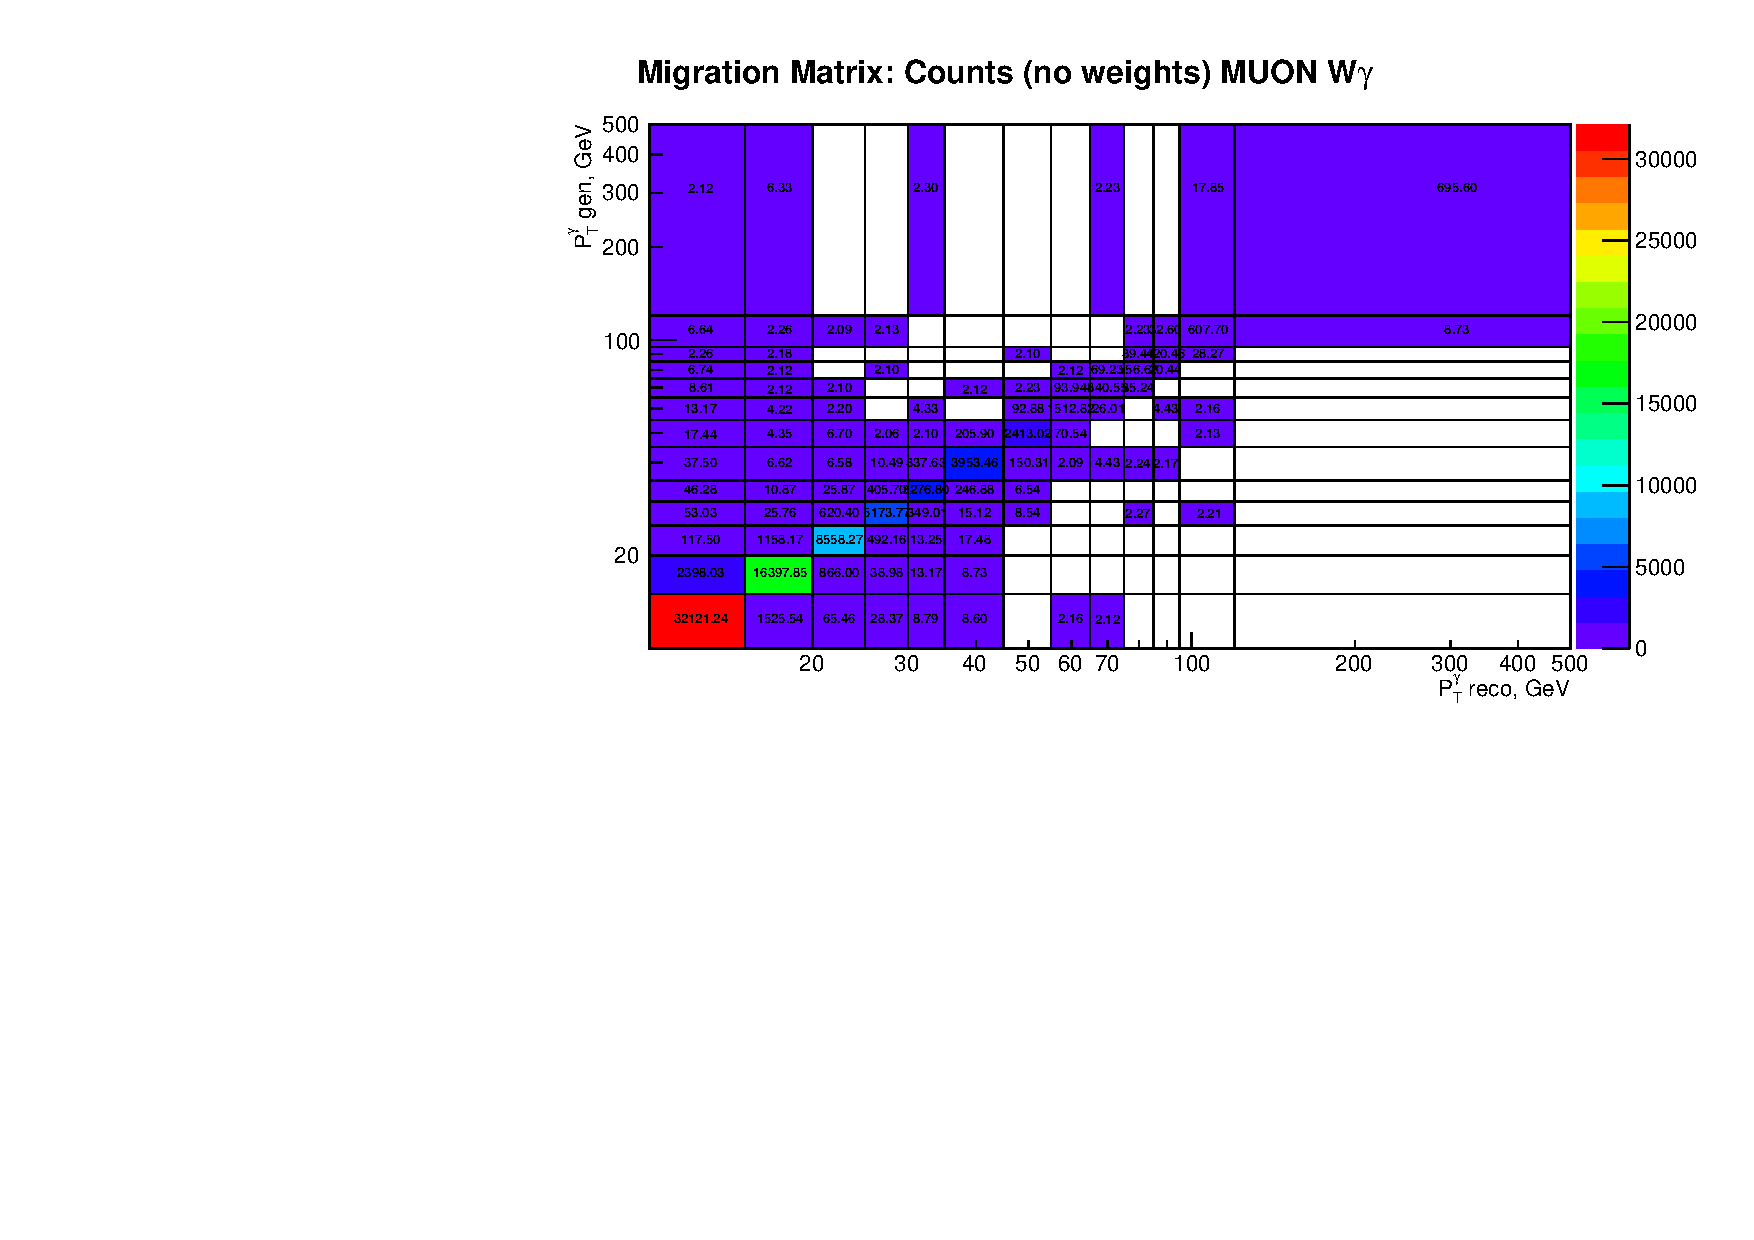
\includegraphics[width=0.90\textwidth]{../figs/figs_v11/MUON_WGamma/Constants/cMigrMatrix_MUON_WGamma__yield_pm_stat.pdf}\\
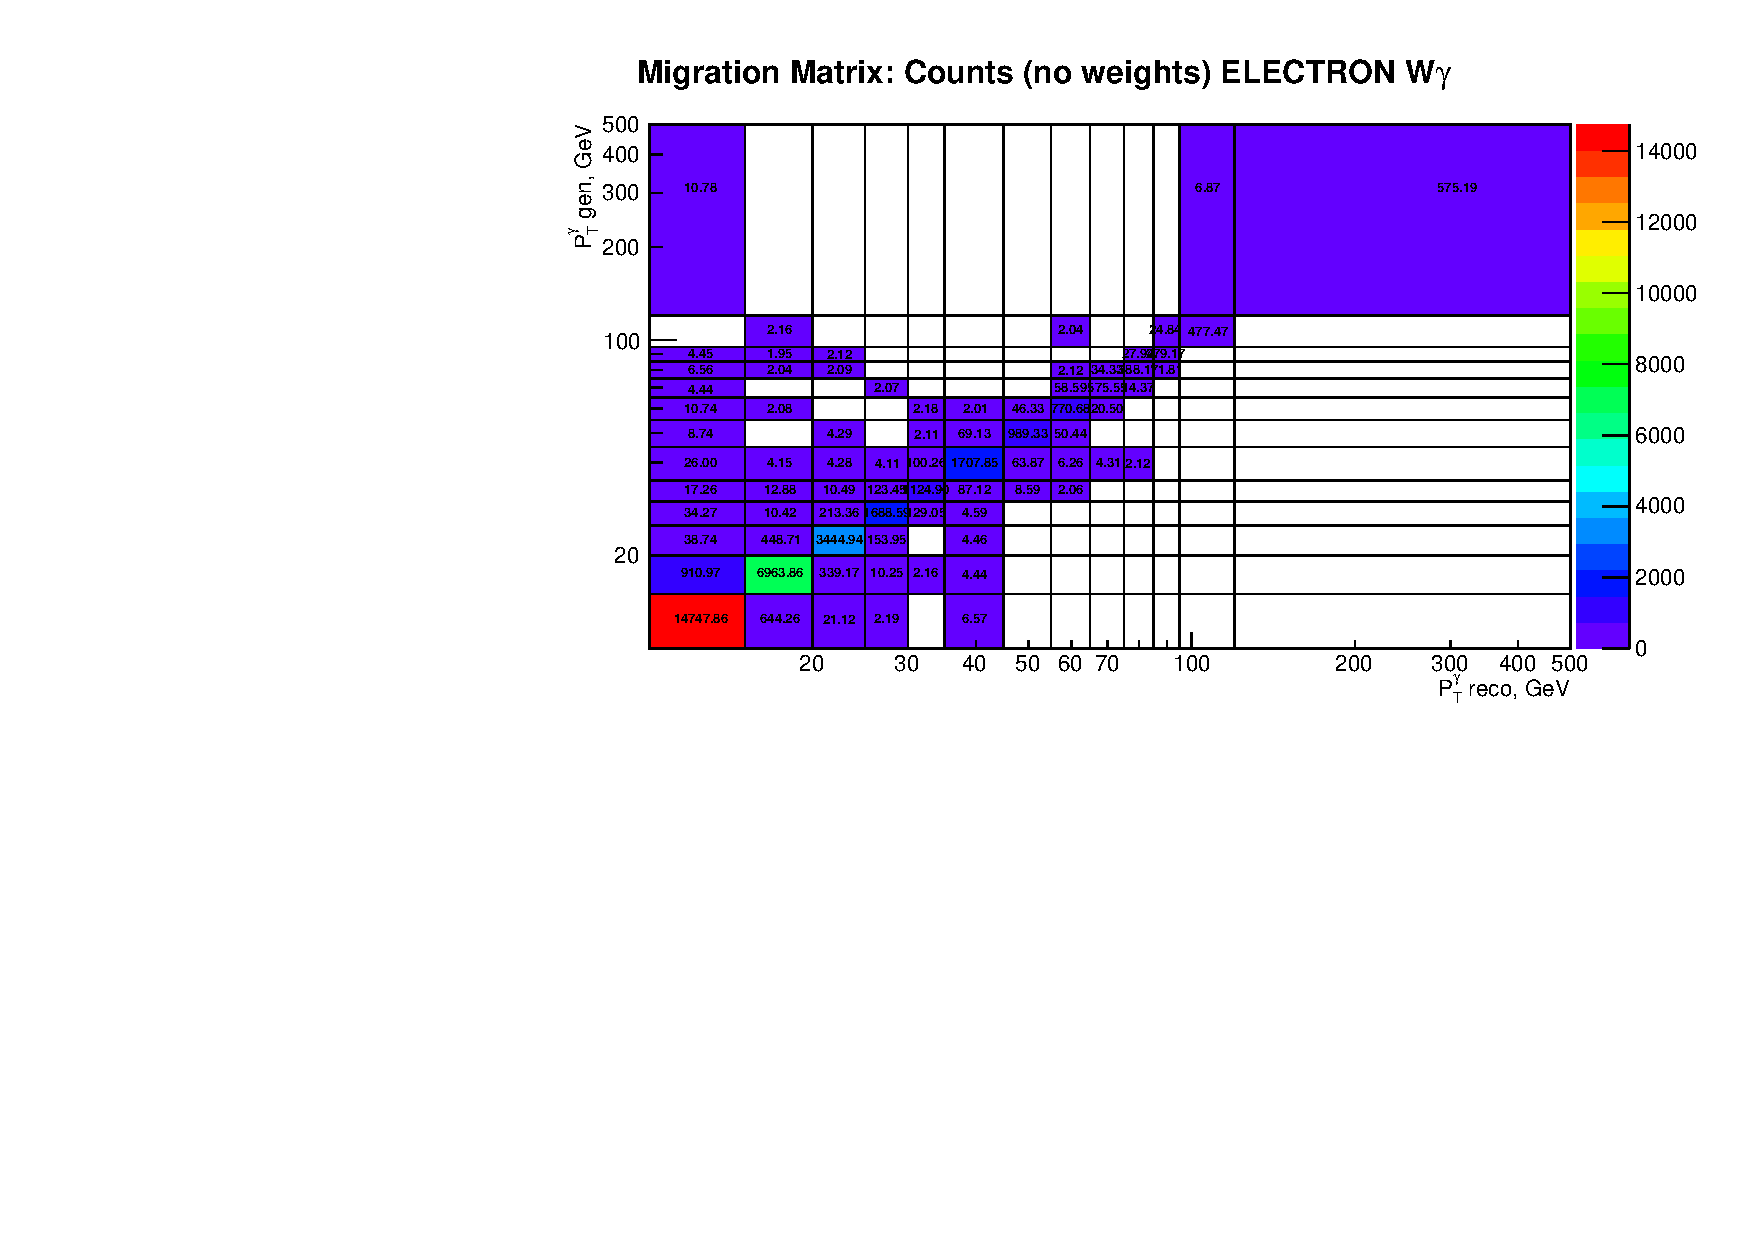
\includegraphics[width=0.90\textwidth]{../figs/figs_v11/ELECTRON_WGamma/Constants/cMigrMatrix_ELECTRON_WGamma__yield_pm_stat.pdf}
  \caption{Migration matrix derived from the signal MC.}
  \label{fig:migrMatrices_Wg}
  \end{center}
\end{figure}

\begin{figure}[htb]
  \begin{center}
   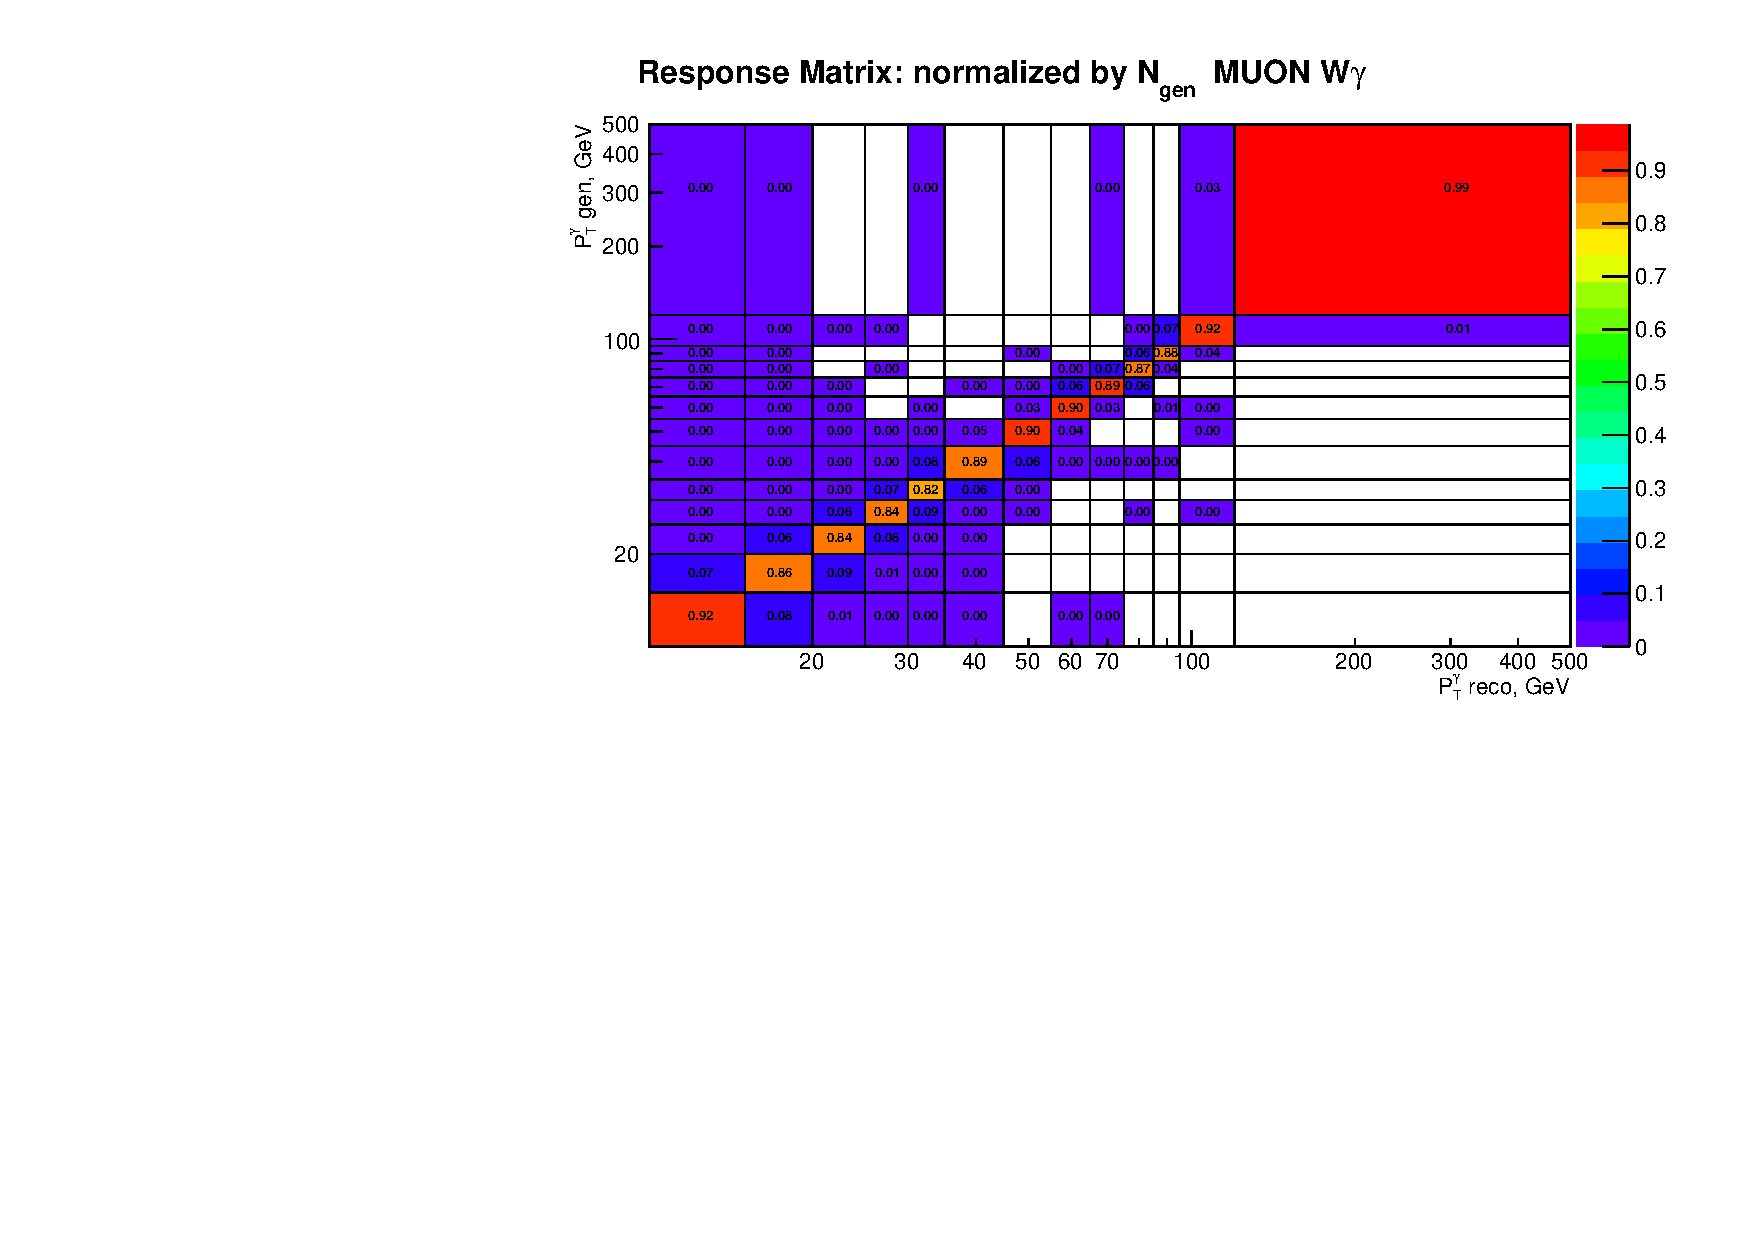
\includegraphics[width=0.90\textwidth]{../figs/figs_v11/MUON_WGamma/Constants/cResponseMatr_MUON_WGamma__yield_pm_stat.pdf}\\
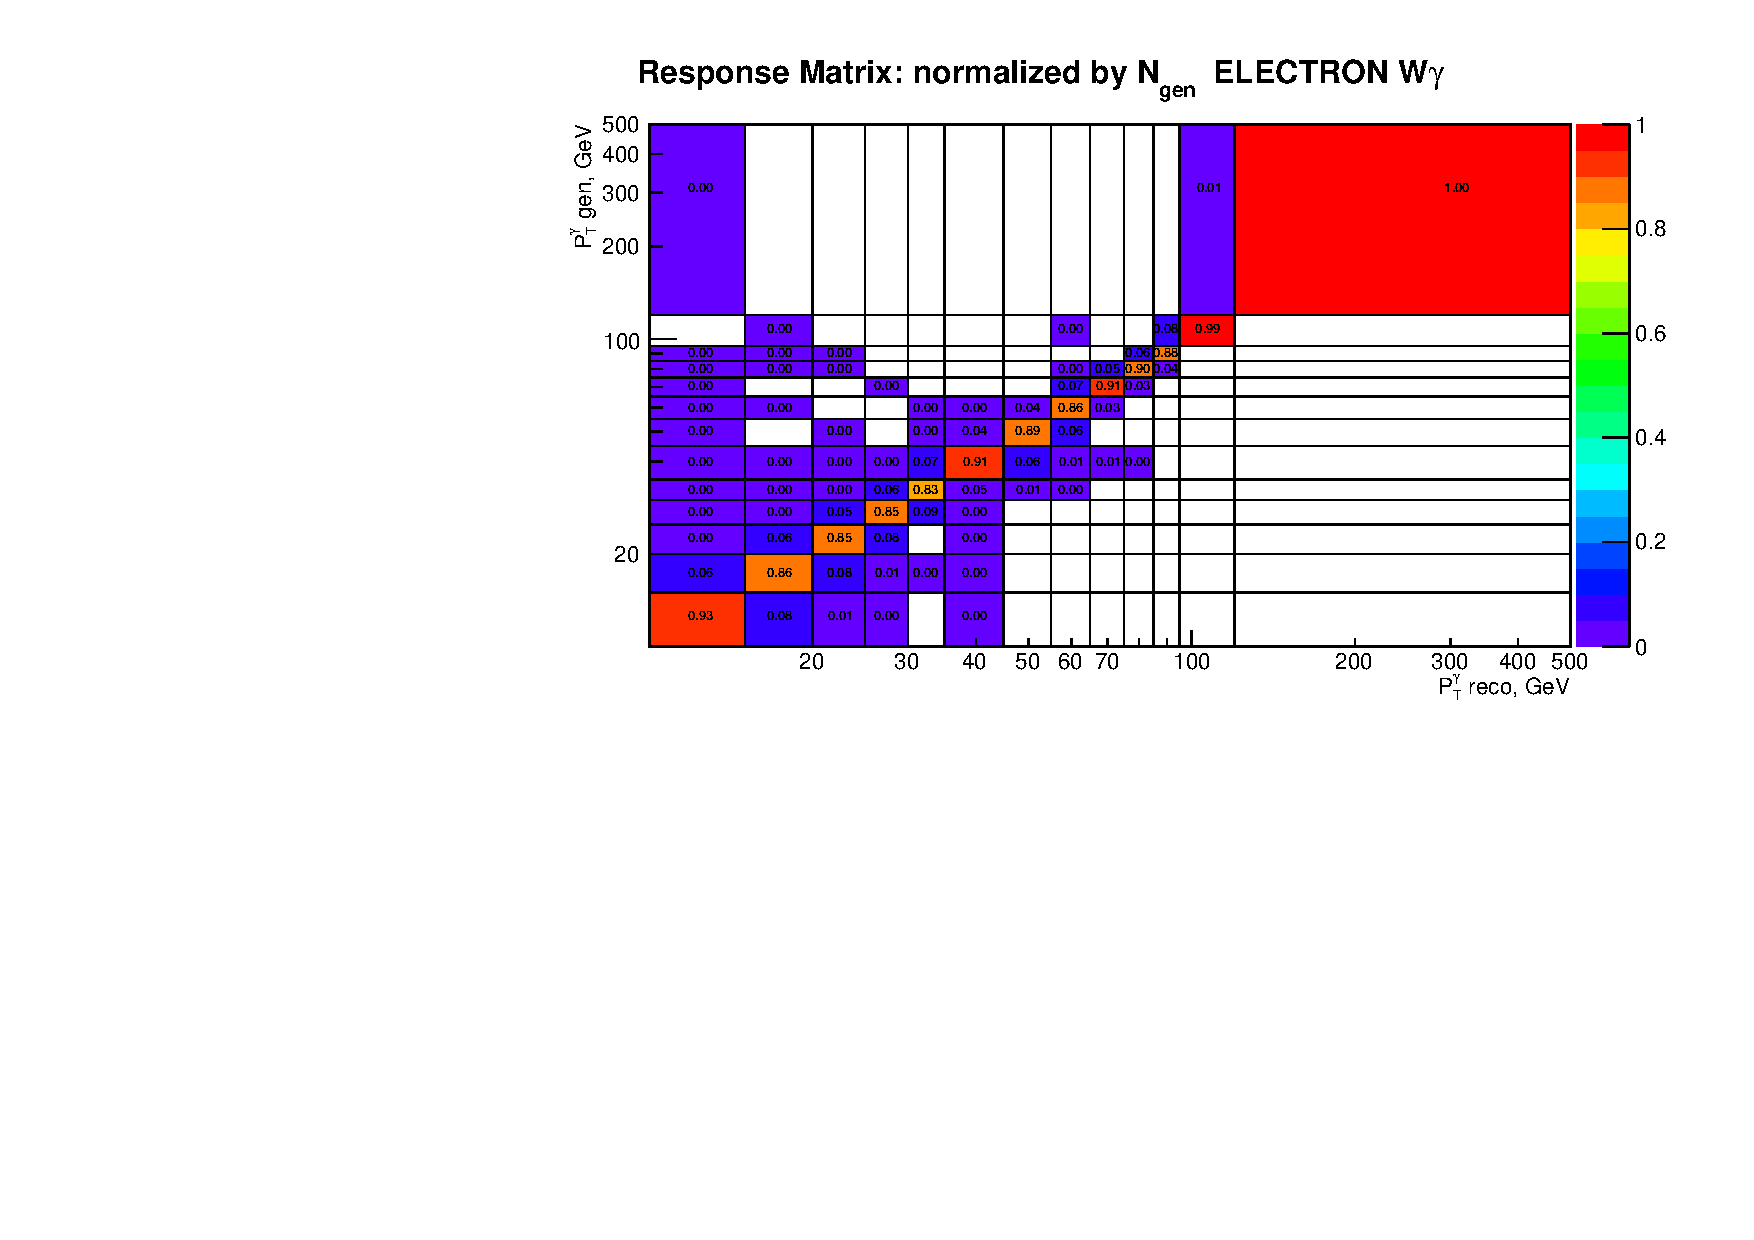
\includegraphics[width=0.90\textwidth]{../figs/figs_v11/ELECTRON_WGamma/Constants/cResponseMatr_ELECTRON_WGamma__yield_pm_stat.pdf}
  \caption{Response matrix derived from the signal MC.}
  \label{fig:respMatrices_Wg}
  \end{center}
\end{figure}

\begin{figure}[htb]
  \begin{center}
   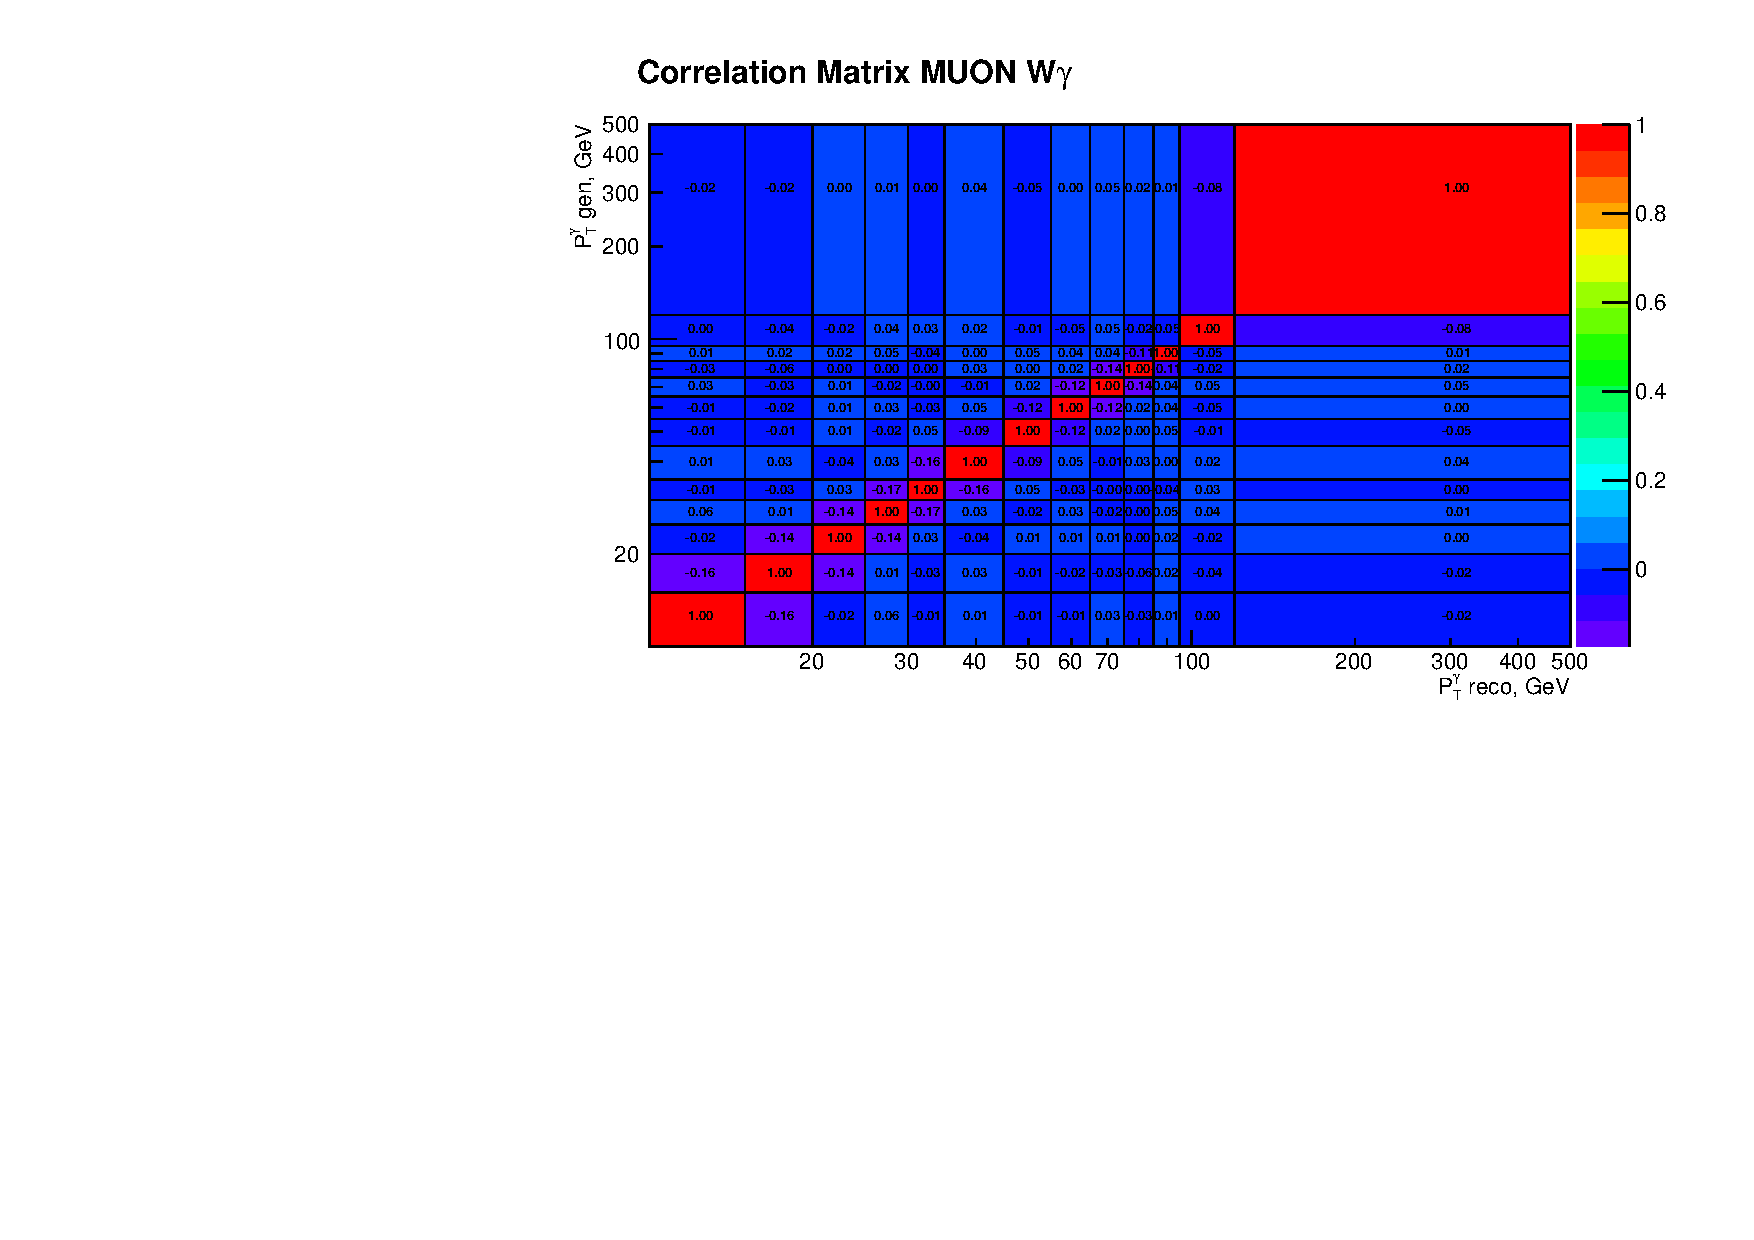
\includegraphics[width=0.90\textwidth]{../figs/figs_v11/MUON_WGamma/Constants/matrCorrelation_yield_pm_stat.pdf}\\
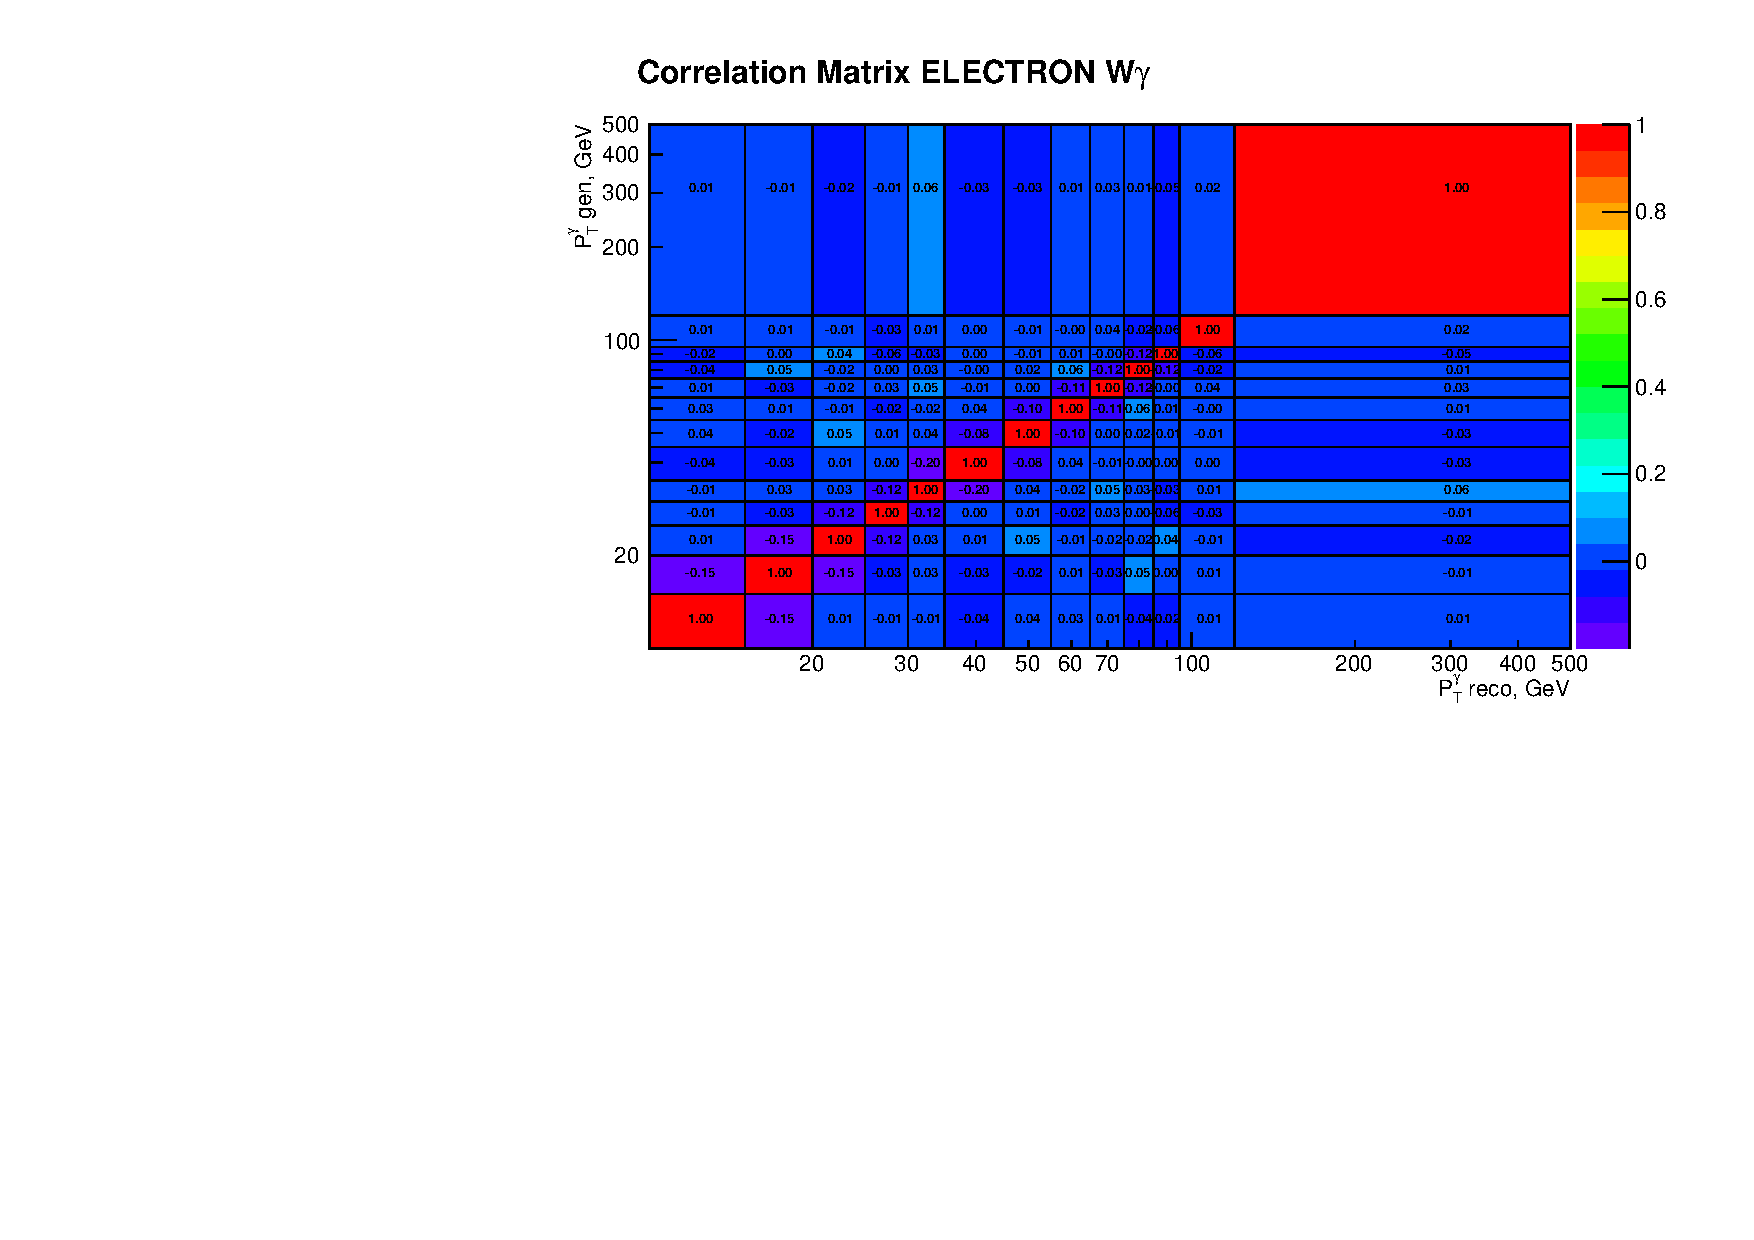
\includegraphics[width=0.90\textwidth]{../figs/figs_v11/ELECTRON_WGamma/Constants/matrCorrelation_yield_pm_stat.pdf}
  \caption{Correlation Matrices.}
  \label{fig:corrMatrices_Wg}
  \end{center}
\end{figure}

%[1] https://indico.cern.ch/event/322577/ 
%[2] https://twiki.cern.ch/twiki/bin/view/CMS/TwikiSMP-GENRecommendations\#Unfolding\_How\_to

% WHAT IS MC CLOSURE CHECK

\begin{table}[h]
  \scriptsize
  \begin{center}
  \caption{Unfolding, MC closure test. MUON WGamma}
  \begin{tabular}{|c|c|c|c|c|}
  bin &  yields &   yields &  unfolded &  unfolded \\ \hline
   limits &  gen-level & rec &  inversion &  D'Agostini \\ \hline
10 -  15 &     $33888\pm 273$ &     $37074\pm 286$ &     $36226\pm206$ &     $36222\pm204$ \\ \hline
 15 -  20 &     $19736\pm 207$ &     $19181\pm 203$ &     $19612\pm171$ &     $19619\pm169$ \\ \hline
 20 -  25 &     $10364\pm 149$ &     $10171\pm 148$ &     $10358\pm122$ &     $10354\pm119$ \\ \hline
 25 -  30 &     $6254\pm 116$ &     $6156\pm 115$ &     $6233\pm96$ &     $6234\pm96$ \\ \hline
 30 -  35 &     $4026\pm  93$ &     $4007\pm  93$ &     $4010\pm81$ &     $4010\pm78$ \\ \hline
 35 -  45 &     $4516\pm  99$ &     $4461\pm  98$ &     $4502\pm79$ &     $4502\pm79$ \\ \hline
 45 -  55 &     $2731\pm  77$ &     $2680\pm  76$ &     $2724\pm57$ &     $2724\pm60$ \\ \hline
 55 -  65 &     $1662\pm  60$ &     $1686\pm  61$ &     $1655\pm45$ &     $1655\pm46$ \\ \hline
 65 -  75 &     $987\pm  46$ &     $945\pm  45$ &     $979\pm38$ &     $979\pm35$ \\ \hline
 75 -  85 &     $659\pm  38$ &     $638\pm  37$ &     $654\pm30$ &     $653\pm30$ \\ \hline
 85 -  95 &     $495\pm  33$ &     $480\pm  32$ &     $489\pm27$ &     $489\pm25$ \\ \hline
 95 - 120 &     $664\pm  38$ &     $663\pm  38$ &     $661\pm28$ &     $661\pm28$ \\ \hline
120 - 500 &     $726\pm  40$ &     $704\pm  39$ &     $720\pm26$ &     $720\pm27$ \\ \hline
500 - 2000 &     $2\pm   2$ &     $2\pm   2$ &     $2\pm1$ &     $2\pm1$ \\ \hline
  \end{tabular}
  \label{tab:unf_mc_closure_MUON_WGamma}
  \end{center}
\end{table}

\begin{table}[h]
  \scriptsize
  \begin{center}
  \caption{Unfolding, MC closure test. ELECTRON WGamma}
  \begin{tabular}{|c|c|c|c|c|}
  bin &  yields &   yields &  unfolded &  unfolded \\ \hline
   limits &  gen-level & rec &  inversion &  D'Agostini \\ \hline
 10 -  15 &     $16025\pm 185$ &     $16849\pm 190$ &     $17117\pm143$ &     $17116\pm141$ \\ \hline
 15 -  20 &     $8246\pm 131$ &     $8111\pm 130$ &     $8194\pm109$ &     $8196\pm108$ \\ \hline
 20 -  25 &     $4093\pm  92$ &     $4046\pm  92$ &     $4083\pm75$ &     $4082\pm74$ \\ \hline
 25 -  30 &     $2080\pm  66$ &     $1987\pm  64$ &     $2072\pm55$ &     $2072\pm55$ \\ \hline
 30 -  35 &     $1387\pm  54$ &     $1361\pm  54$ &     $1378\pm47$ &     $1378\pm46$ \\ \hline
 35 -  45 &     $1925\pm  64$ &     $1886\pm  63$ &     $1915\pm51$ &     $1915\pm50$ \\ \hline
 45 -  55 &     $1124\pm  49$ &     $1108\pm  48$ &     $1116\pm37$ &     $1116\pm38$ \\ \hline
 55 -  65 &     $855\pm  42$ &     $892\pm  43$ &     $848\pm33$ &     $848\pm34$ \\ \hline
 65 -  75 &     $655\pm  38$ &     $635\pm  37$ &     $649\pm30$ &     $649\pm28$ \\ \hline
 75 -  85 &     $447\pm  32$ &     $433\pm  32$ &     $442\pm24$ &     $442\pm24$ \\ \hline
 85 -  95 &     $316\pm  27$ &     $316\pm  27$ &     $311\pm21$ &     $311\pm20$ \\ \hline
 95 - 120 &     $507\pm  34$ &     $484\pm  33$ &     $501\pm23$ &     $501\pm23$ \\ \hline
120 - 500 &     $593\pm  37$ &     $575\pm  36$ &     $587\pm23$ &     $587\pm24$ \\ \hline
500 - 2000 &     $4\pm   3$ &     $4\pm   3$ &     $4\pm2$ &     $4\pm2$ \\ \hline
  \end{tabular}
  \label{tab:unf_mc_closure_ELECTRON_WGamma}
  \end{center}
\end{table}
